%Correct the file name.
%X: book number
%Y: part number
%ZZZ: page number in three digits. So page 3 would be 003.

\documentclass[11pt]{amsbook}

%\usepackage{../HBSuerDemir}
\usepackage{../Ceyhun}	
\usepackage{../amsTurkish}	% ------------------------


\begin{document}

% ++++++++++++++++++++++++++++++++++++++
\hPage{Feyzioglu-047}
% ++++++++++++++++++++++++++++++++++++++
\begin{lemma}(Euclid's lemma): 
\textit{Let a,b,p be integers. If p is prime and $p| ab$, then $p|a$ or $p|b$.}
\end{lemma}
\begin{proof}
If $p|a$, the lemma is proved. If $p\nmid a$, then (a;p) = 1 by Lemma 5.14. and, since $p|ab$, we get $p|b$ by Theorem 5.12 (with p,a,b in place of a,b,c, respectively). 
\end{proof}
\begin{lemma}
\textit{Let $a_{1},a_{2}, ... ,a_{n}p$ be integers.If p is prime and $p|a_{1}a_{2}...a_{n}$, then $p|a$ or $p|a$ or...or $p|a_{n}$.
}
\end{lemma}
\begin{proof}
This follows from Euclid's lemma by a routine induction argument. The details are left  to the reader.
\end{proof}

We can now prove uniqueness aside from trivial variations.

\begin{theorem}(fundamental theorem of arithmetic):
\textit{Every integer, which is not zero or a unit, can be expressed as a product of prime numbers in a unique way,apart from the order of the factors and ambiguity of associate numbers.}
\end{theorem}
\begin{proof}
Let $n\in \mathbb{Z}, n\neq 0, n\neq$ unit.By theorem 5.13, n can be expressed as a product of prime numbers.We must show uniqueness.This will be done by induction on $|n| \in \mathbb{Z} $.Given two decompositions 

\begin{center}
$p_{1}p_{2}...p_{r}=n=q_{1}q_{2}...q_{s}$
\end{center}

of n into prime factors, we have to show that

\begin{center}
r=s
\end{center}

and that 

\begin{center}
$p_{1},p_{2},...p_{r}$ are in some order associate to $q_{1},q_{2},...q_{s}$
\end{center}

Assume first $|n|$ = 2.Then n = 2 or n = -2 is prime and n = $\mp2$ is the unique representation of n as a product of prime numbers (having only one factor).So the theorem is true for n if $|n|$=2.

Now we make the inductive hypothesis that $|n|>$2 and that the theorem is true for all k $\in \mathbb{Z}$ with $2\leqslant |k| \leqslant$n-1,and prove it for n.
\end{proof}

\end{document}  

%==== templates ====

%==== environments ====

%\begin{figure}[htb]
%	\centering
%	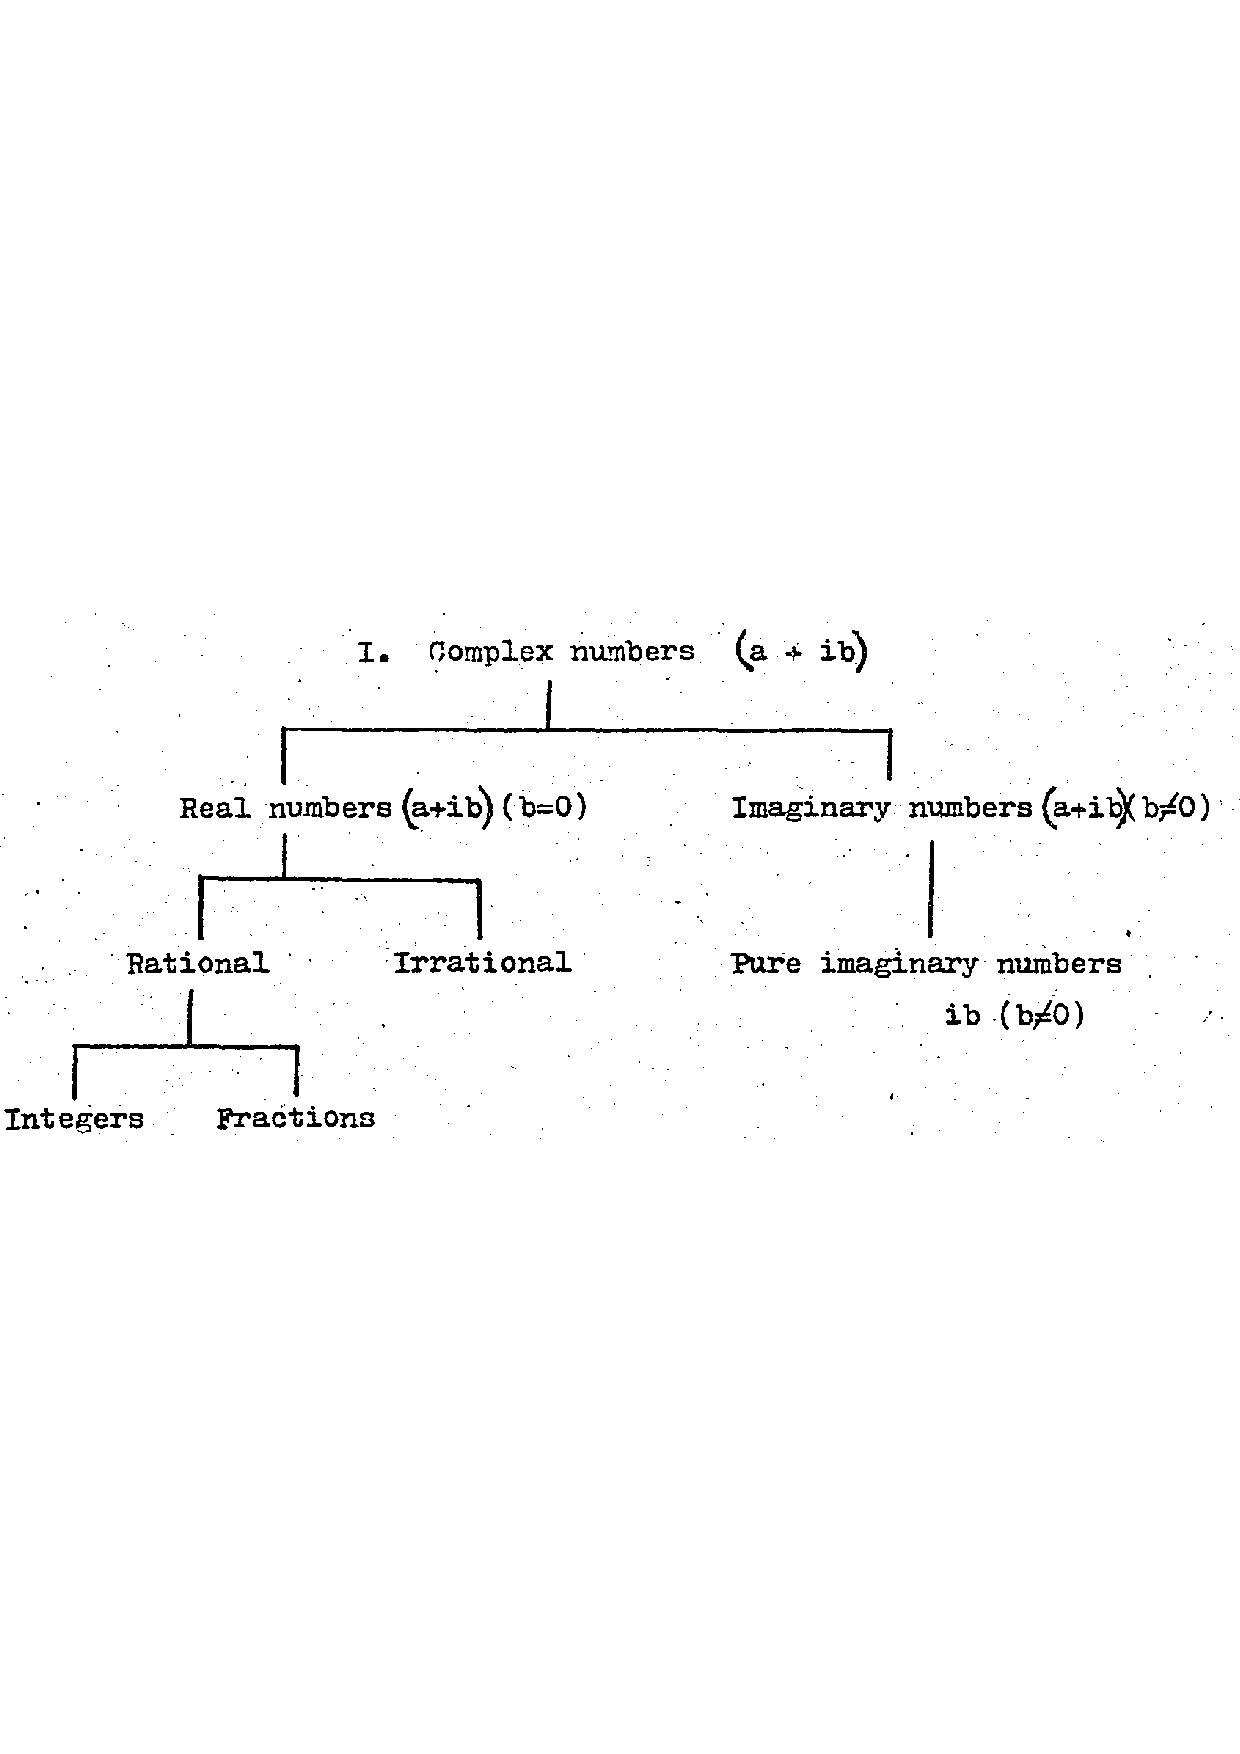
\includegraphics[width=0.9\textwidth]{images/SD-1-1p15A}
%	\caption{Classification of complex numbers}
%	\label{fig:classificationOfComplexNumbersA}
%\end{figure}

%\begin{center}
%\begin{tabular}{cc}
%\end{tabular}
%\end{center}

%\begin{exmp}
%\begin{hSolution}
%\end{hSolution}
%\end{exmp}

%\begin{hEnumerateAlpha}
%\end{hEnumerateAlpha}

%\begin{hEnumerateRoman}
%\end{hEnumerateRoman}

%$
%\begin{bmatrix}
%\end{bmatrix}
%$

%\frac{aaaa}{bbb}
%\frac{a_{n}}{b_{n}}
%\left( aaaa \right)
%\Longrightarrow

%\begin{multicols}{2}
%	bb
%\columnbreak
%	aa
%\end{multicols}
